\begin{table*}[t]
\centering
\caption{Reported BraTS T2$\to$FLAIR results. Values are copied from each paper's table; protocols differ, so rows from different papers are \emph{not} comparable. SSIM in \%. Selected rows; FADM and ResViT SSIM converted from $[0,1]$. $^{\ddagger}$: digits identical (or one digit apart) to a row of the SelfRDB paper's Table~2 obtained under a different protocol, in two cases for a differently named method (WRB ``BBDM'' = SelfRDB ``I$^2$SB''; WRB ``CycleGAN'' mean and SSIM = SelfRDB ``SAGAN'').}
\label{tab:lit}
\footnotesize
\setlength{\tabcolsep}{3pt}
\resizebox{\textwidth}{!}{%
\begin{tabular}{llccl|l}
\toprule
Source & Method & PSNR (dB) & SSIM (\%) & Source table & Protocol of the source \\
\midrule
WRB~\cite{yang2026wrb} & pix2pix$^{\ddagger}$ & 24.85$\pm$1.57 & 83.36$\pm$3.11 & Tab.~1 & BraTS'21, 25/5/10 subj.; slices 27--126; per-slice $[0,1]$; foreground mask; per-slice stats \\
 & CycleGAN$^{\ddagger}$ & 27.08$\pm$3.42 & 87.59$\pm$2.93 &  &  \\
 & BBDM$^{\ddagger}$ & 25.92$\pm$2.00 & 83.51$\pm$4.05 &  &  \\
 & DDPM$^{\ddagger}$ & 26.90$\pm$1.84 & 87.86$\pm$2.85 &  &  \\
 & SelfRDB & 26.84$\pm$1.88 & 90.59$\pm$2.79 &  &  \\
 & WRB & 27.51$\pm$1.00 & 91.33$\pm$2.07 &  &  \\
\midrule
FADM~\cite{jiang2025fadm} & CycleGAN & 19.21$\pm$2.61 & 82.7$\pm$5.7 & Tab.~2 & BraTS'21, 80/10/10; 70 slices/subj.; resized to 256; norm., mask, unit not reported \\
 & pix2pix & 25.91$\pm$3.72 & 83.7$\pm$4.7 &  &  \\
 & SR3 & 27.49$\pm$2.01 & 86.9$\pm$3.7 &  &  \\
 & I$^2$SB & 29.21$\pm$2.44 & 93.7$\pm$2.4 &  &  \\
 & FADM & 30.85$\pm$1.34 & 95.8$\pm$2.5 &  &  \\
\midrule
SelfRDB~\cite{arslan2025selfrdb} & pix2pix & 26.85$\pm$1.57 & 86.36$\pm$3.11 & Tab.~2 & BRATS, 25/10/20; 100 slices/subj.; volume mean-norm.; mask not stated \\
 & SAGAN & 27.08$\pm$1.57 & 87.59$\pm$2.93 &  &  \\
 & DDPM & 26.90$\pm$1.84 & 87.86$\pm$2.85 &  &  \\
 & SynDiff & 27.77$\pm$1.77 & 89.62$\pm$2.87 &  &  \\
 & I$^2$SB & 25.92$\pm$2.00 & 83.51$\pm$4.05 &  &  \\
 & SelfRDB & 27.98$\pm$1.80 & 90.01$\pm$2.70 &  &  \\
\midrule
SynDiff~\cite{ozbey2023syndiff} & cGAN & 27.41$\pm$0.78 & 88.48$\pm$1.45 & Tab.~III & BRATS, 25/10/20; 100 slices/subj.; \emph{unpaired} training \\
 & DDPM & 25.49$\pm$0.60 & 84.71$\pm$1.40 &  &  \\
 & SynDiff & 28.17$\pm$0.90 & 90.44$\pm$1.48 &  &  \\
\midrule
ResViT~\cite{dalmaz2022resvit} & pix2pix & 23.15$\pm$1.93 & 86.9$\pm$1.6 & Tab.~V & BRATS, 25/10/20; 100 slices/subj.; norm.\ and mask not reported \\
 & pGAN & 24.01$\pm$1.15 & 86.4$\pm$1.4 &  &  \\
 & ResViT & 24.97$\pm$1.07 & 87.0$\pm$1.4 &  &  \\
\midrule
D3Bridge~\cite{xie2026d3bridge} & D3Bridge & 26.00 & 89.57 & README & BraTS'21, 25/5/10 (repository README only; no paper found) \\
\bottomrule
\end{tabular}}
\end{table*}

\begin{figure}[t]
\centering
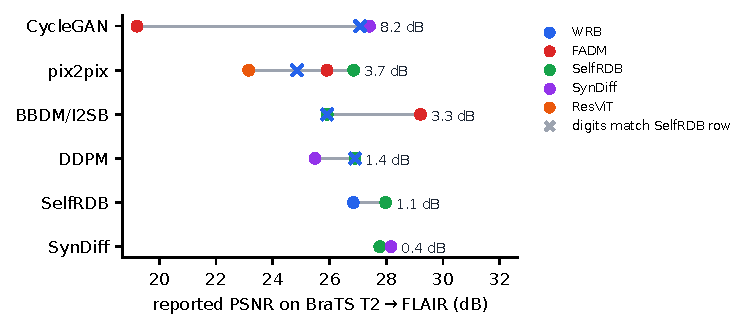
\includegraphics[width=\columnwidth]{figures/literature_protocols.pdf}
\caption{The same method as reported by different papers on BraTS T2$\to$FLAIR (crosses: WRB rows whose digits match a SelfRDB-paper row; BBDM and I$^2$SB share a row because WRB's ``BBDM'' equals SelfRDB's ``I$^2$SB''; SynDiff's own numbers are from unpaired training). The spread for one method with paired training (3.7~dB for pix2pix, 3.3~dB for BBDM/I$^2$SB; the 8.2~dB CycleGAN spread mixes paired and unpaired training) is as large as the gaps the papers report between methods, so the protocol, not the method, dominates cross-paper differences.}
\label{fig:lit}
\end{figure}

Table~\ref{tab:lit} and Fig.~\ref{fig:lit} make three points. First, the protocols differ in subject split (40 to 100 subjects, 10 to 20 test subjects), slice selection, resizing versus padding, normalization, masking and statistic unit, and several of these are not reported at all. Second, the same method moves by several decibels between papers (pix2pix from 23.15 to 26.85~dB; I$^2$SB from 25.92 to 29.21~dB), which is larger than most reported method-to-method gains. Third, several baseline rows of WRB's T2$\to$FLAIR table are digit-identical to rows of the SelfRDB paper, which used a different split (55 instead of 40 subjects), and in two cases the rows are attributed to differently named methods; we could not find a protocol under which both would be measured. We therefore do not rank our results against published numbers. Instead we retrain the reproducible baselines (pix2pix, SelfRDB) on our split, and we report a literature-protocol run only to calibrate how far the protocol moves PSNR.
